% Following magic comments allow for compilation of root file
% !TEX root = ../../../../temp_manuscript.tex

\chapter{Discussion}\label{chap:discussion}
\begin{ChapterAbstractNoTitle}
\end{ChapterAbstractNoTitle}
In this thesis, I showed the potential of automated image analysis of glioma for several different tasks.
Most prominently, I developed machine learning methods that predict the genetic status of glioma from preoperative \gls{MRI} scans (\cref{chap:LGG1p19q,chap:prognosais}).
I also used computational methods to evaluate potential observer-independent imaging markers (\cref{chap:HGGLocation,chap:LGGLocation}), developed machine learning methods to help with the initial stages of research (\cref{chap:DDS}), and the segmentation of glioma (\cref{chap:prognosais}).
In this chapter, I discuss the main findings of this thesis, highlight my contributions, and provide an outlook on the future clinical impact of these methods and potential future research directions.

\section{Radiomics performance benchmarks}

An important barrier for clinical acceptance of radiomics methods is their predictive performance.
In \cref{chap:LGG1p19q,chap:prognosais}, I developed two machine learning methods that predict the genetic features of glioma.
Although these methods successfully predicted the genetic features, their performance was considered insufficient for clinical use.
However, there is no generally accepted threshold for sufficient clinical performance, which makes it hard to determine what the main focus of performance improvement should be.
For example, it is possible to try and improve the overall performance, but in some cases it might be more interesting to improve the performance in specific subgroups.

The observer-independency and speed of machine learning methods make it easy to measure their performance on different datasets.
However, the ease of performance measurement and abudance of reported achieved performances has led to (perhaps unrealistically) high expectations of these methods.
First of all, the performance of radiomics methods is always compared to a golden standard that is derived through some other method (e.g. through the analysis of a biopsy sample in the case of genetic features).
The machine learning methods will never (directly) outperform these golden standard methods; in that sense, the performance will never be acceptable, since the currently available method is already better.
Of course, the radiomics methods have a different starting point from which they try to derive the same information (e.g. a scan instead of a tumor sample to predict the genetic features).
Thus, the radiomics methods might need to be compared against a different benchmark than always being compared to the golden standard ground truth.
For example, in \cref{chap:LGG1p19q}, we did not reach perfect performance compared to the ground truth obtained from tumor tissue analysis.
However, when we compared our method with clinical experts, who used the same data as was available to the algorithm, we found that our algorithm was able to outperform some of them.
Thus, based on this benchmark, the performance might already be acceptable for clinical use, since it can improve over the current situation.

The advantage of radiomics methods is that they can provide the information earlier in the treatment trajectory than the gold standard method, and often do so based on data that is easier to obtain (a scan vs a tumor sample).
However, not all institutes have the resources required to use the golden standard methods, especially in underprivileged countries \autocite{santosh2019india}.
With the addition of more genetic features in the glioma categorization, the price of the equipment needed to analyze these features also increases, and even for privileged institutes that have access to the required equipment it might not be cost-effective to analyze all \glspl{tumor}\autocite{malzkorn2016practical,dewitt2017costIDH}.
This makes these golden standard methods, although preferable for their accuracy, infeasible as the de facto standard.
In these cases, radiomics methods can be a cheap and easy-to-use solution, which, although having suboptimal performance, can still improve over the current situation of having no information about the molecular and histological features.
This also means that the benchmark with which the radiomics methods are compared could differ between institutes.
For example, the experts with which we compared our method in \cref{chap:LGG1p19q} were highly specialized in glioma and came from an institute specialized in glioma.
Thus, it is likely that not all institutes have acces to the same lever of expertise, which lowers the bar for clinically acceptable performance of radiomics methods in some institutes, and the performance that some of the current methods achieve might already improve the patient treatment.

Therefore, there might also need to be a shift in the way radiomics is positioned.
Currently, it is often presented as a method that can replace a certain (currently used) golden standard method or even replace clinical experts.
Although this might become a reality in the long run, at the moment this seems rather unlikely.
Perhaps radiomics is better viewed as a way to democratize clinical expertise.
The methods can be developed using the latest insights and expertise available at privileged institutes, and this knowledge can then be distributed to institutes that normally would not have access to it.


\section{Uncertainty in the ground truth}

An important aspect for all machine learning methods is the uncertainty in the ground truth.
I distinguish two categories of uncertainty: The first category is an imperfect, but observer-independent ground truth method, the second category is an observer-dependency in the ground truth.

The genetic analysis of tumor tissue is imperfect (and also contains some observer dependency, although this could be eliminated).
For example, when comparing multiple methods to determine the \gls{IDH} status of \gls{tumor} tissue, these methods are not always in agreement \autocite{pyo2016concordance}.
As a result of this uncertainty in the golden standard, the ground truth used to train and evaluate machine learning methods probably contains errors.
Of course, in these cases it is still unknown what the \say{true} ground truth is, since there is no way too \per{100} accurately determine it, making it impossible to gain a true feeling for the uncertainty in the ground truth.
The uncertainty can be larger for some ground truths than for others, for example the accuracy for the analysis of the \gls{MGMT} status is quite low \autocite{wang2017mgmt}.
The uncertainty for a specific output is important to take into account during the development of a machine learning model, since it might not actually possible to properly train a model if the uncertainty in the ground truth is too large.

Another aspect is the observer-dependency of some ground truths.
For example, in the case of tumor segmentation it is not possible to determine a \say{true} ground truth, it will always depend on the observer that made it.
In cases where the ground truth is observer-dependent, striving for the best performing algorithm might be unrealistic, since the ground truth could be less accurate than the predictions.
For example, when comparing segmentation from multiple observers, a whole \gls{tumor} mean DICE score of 0.85 was found, which is very close our DICE score of 0.84 achieved in \cref{chap:prognosais} \autocite{menze2015brats}.
Therefore, it might be hard to improve the performance further, especially if ground truth segmentation of multiple observers are used to train the algorithm.
In this way, automated methods can be very helpful for \gls{tumor} segmentation, as they homogenize the \gls{tumor} segmentations.
However, what a segmentation contains is based on personal and institutional preferences, thus multiple methods might need to be trained to achieve the same goal of \gls{tumor} segmentation for different institutes.

\section{Input data assumptions}

In this thesis we have studied glioma.
Here, the assumption was always made that the scans that were used actually were scans of glioma patients.
When patients first come into the clinic with complaints, there is still a variety of options that could cause the same symptoms as glioma, without the patient actually having a glioma.
Therefore, the diagnosis of a glioma usually involves \gls{CT} and/or \gls{MRI} scans.
However, this means that these scans need to be interpreted to determine what the anomaly on the scan actually is, and sometimes it can be wrongly interpreted as a glioma.
Thus, the methods presented in \cref{chap:LGG1p19q,chap:prognosais} are not fully automated, since these kinds of interpretations still manually need to be made upstream.
To make a fully automatic pipeline, machine learning algorithms can be developed that distinguish between different types of brain conditions, for example between glioma and metastasis \autocite{chen2019metastatic}.
This interpretation upstream can also result in non-glioma scans being fed into the machine learning algorithms, in which case it will of course still make its predictions, as it cannot indicate that the scan did not contain a glioma.

It is important to consider, and explicitly state, what assumptions about the input data are made.
For example, in \cref{chap:LGG1p19q} we assumed that the scans were of presumed \gls{LGG}, based on the visual appearance of these glioma in the scan.
Thus, this adds another upstream analysis step which can cause errors in the input data, and it restricts the applicability of these algorithms, since clinical expertise is needed for the interpretation of the scans.
Therefore, in \cref{chap:prognosais} we made no such assumptions, instead we included any type of glioma.
This generalization reduces the amount of upstream steps, reducing the potential for errors made in the evaluation of the data.
However, a further generalization to also include non-glioma scans would mean that these algorithms need to predict multiple, unrelated outputs.
For example, one output can still be the \gls{IDH} mutation status, while another output is whether a scan shows a brain infarct, in which case the \gls{IDH} mutation is nonsensical.
Thus, the machine learning methods should be as generalizable as possible to reduce the amount of upstream analysis that needs to be done, while making sure that the predictions of the model remain coherent.
If the outputs are not coherent, the tasks should be split up into several models.


\section{Interpretability of machine learning methods}

Another important barrier for the acceptance of machine learning methods is their lack of interpretability.
Deep learning methods especially are considered black boxes since there is no explicit knowledge on what imaging features these methods base their prediction on.
Thus, it is hard to trust the predictions of these methods, especially when considering that the clinical experts and the patient probably want an explanation as to why a certain treatment decision is made.

In \cref{chap:LGG1p19q,chap:prognosais,chap:DDS} we  tried to provide some insight into the machine learning methods.
In \cref{chap:prognosais,chap:DDS} we did so by showing attention maps and convolution filter outputs, and in \cref{chap:LGG1p19q} we looked at the relative importance of different features.
Although in this way we can provide some insight into the machine learning methods, this is only very globally and lacks an explanation as to why certain imaging features are used in the prediction.
Although a lot of research is focusing on methods that can provide additional insight into these methods, the question remains whether human-interpretable explanations of machine learning methods will be available in the near future \autocite{zhang2018interpretable}.
This creates distrust for these algorithms, since even if it can be shown that an algorithm is looking at the correct part of the scan (i.e. in the tumor and not somewhere outside the brain), the algorithm might consider it for the wrong reasons.
It is easy to attach our own explanation to these methods if we see them focusing on particular parts, but this can easily lead to misinterpretations.
A method that can explain why a deep learning network looks at a specific part of a scan would not only create more trust in the algorithms, as the predictions can now be verified, it can also help to develop new and better ones.
If a sample is wrongly predicted, but the algorithm can explain why it looked at certain parts, it might be possible to redesign the method to make sure that the method looks at the correct parts of the scans.

\section{Deep learning models}

An important technical limitation that deep learning methods face is the limited amount of memory available on GPUs, which constrains the size of deep learning models.
In \cref{chap:prognosais}, I developed a method that can fit a large model, while also using the full 3D scan as an input.
However, this model pushed the limits of the GPU memory, and the model could not be larger on the GPU available for this research.
On the one hand this limitation leads to a critical evaluation of what is essential in the model, cutting out the superfluous parts.
On the other hand, larger models might improve the performance of deep learning methods.

Larger models do not always have to contain merely more filters than their smaller counterparts, since more filters might not always lead to better results.
However, models can be extended in other ways, for example some models use the scan at different resolutions, thereby trying to force the model to learn features that are relevant at different scales \autocite{akkus20171p19q}.

Another interesting approach would be to keep the different scan modalities separate during the convolutions.
Currently, the first convolutional layer combines the different modalities into feature maps.
However, keeping the modalities separate deeper into the model may lead to different features being learned.
Of course, one can then also make different paths in the models for different combinations of modalities, where each path learn specific features.
However, this will significantly increase the amount of memory required to train these models.
A schematic of such a model is shown in \cref{fig:discussion_architecture}.
This model contains XXX parameters, XXX as much as the model presented in \cref{chap:prognosais}.

\begin{figure}
\includegraphics[width=\textwidth]{example-image-a}
\caption{Example architecture with pathways for different imaging modalities}\label{fig:discussion_architecture}
\end{figure}

The amount of GPU memory has been increasing, and in the past four years the amount of memory at the same pricepoint has doubled.
Furthermore, new innovations such as half-precision training and parallel training allow for bigger models to be trained using the same amount of memory.
The optimization of current models and methods to make use of these new features can already lead to the use of new model types, although the impact of larger models remains to be seen.
This advance in hardware raises an important ethical question.
If the best performing models can only run on the newest (most expensive) GPUs, this would be a big obstacle in research and in the clinical applicability of these methods.

\section{Imaging}

One of the big challenges for radiomics that use \gls{MRI} scans at the moment is the qualitative nature of \gls{MRI} scans, which does not allow for objective biomarkers.
In recent years quantitative \gls{MRI} has gained in popularity, where using new \gls{MR} sequences allows for the measurement of the true tissue values.
This means that voxel values in these quantitative \gls{MRI} scans now have a meaning, and that the same patient scanned on different scanners should result in the same scan.
This makes the development of new imaging biomarkers and automated methods easier, as they can now use the absolute voxel intensity.
However, quantitative \gls{MRI} sequences are not yet clinically used.

Another important development is the development of new \gls{MRI} sequences.
For example, \gls{DWI} and \gls{PWI} sequences which provide physiological information in addition to the structural information provided by sequences such as \gls{T1} and \gls{T2} used in this thesis.
It has been shown that adding these sequences in radiomics methods provides additional information, and leads to a better performance \autocite{park2020radiomicsdwi,kim2020radiomicsdwi}.
We did not include these sequences in the research in this thesis, as they were not as present four years ago as they are now, thus not enough data was available.
New \gls{MRI} sequences are constantly being developed, for example \gls{CEST}, which provides additional physiological data not present in \gls{PWI} and \gls{DWI}.

However, radiomics will always lack behind in making use of new scan sequences, since a database first needs to be build up with sufficient patients for which these scans are available.
In the case of quantitative \gls{MRI} this problem can be partially solved by using transfer learning.
Transfer learning takes an already trained algorithm, and tries to use the knowledge of that algorithm to make the training of a new algorithm on slightly different, but related, data easier \autocite{shin2016transfer}.
Since there is a relationship between the qualitative and quantitative \gls{MRI}, using transfer learning should minimize the amount of data needed to retrain these algorithms.


\section{Genetics}

In \cref{chap:HGGLocation} we saw that we could find no relationship between the \gls{MGMT} status of a tumor and the location of the tumor within the brain.
Then, in \cref{chap:prognosais}, we also attempted to predict the \gls{MGMT} status from \gls{MRI} scans, now using a deep learning network, where we did not find a relationship with the \gls{MGMT} status either.
A recent study by \citeauthorref{mikkelsen2020mgmt} also could not find a relationship between the \gls{MGMT} status and radiomics features.
In literature, the number of studies that successfully predicted the MGMT methylation status is limited, especially in comparison with the prediction of other genetic statuses.
Studies that did manage to find a correlation might be biased by predicting the IDH status instead.
Therefore, an important questions remains whether the imaging features can determine the MGMT status.

An important development in the field of genomics is the commodity of more advanced genetic analysis machines.
With the introduction of next generation sequencing the results from the genetic analysis become more reliable, which allows for a better training of radiomics models, and also allows for more genes to be analyzed.
In this way, new genes can be discovered that correlate with the aggressiveness of the tumor, and in the future the categorization will most likely be solely dependent on molecular features.
However, this introduces problems for machine learning methods, as they will always lack behind.
If a new gene is discovered that is relevant for glioma, first a database needs to be build up that contains information on this gene.
The model proposed in \cref{chap:prognosais} might form part of the solution to this problem.
By predicting multiple genetic and histological features simultaneously, the method was able to learn relationships between the different features.
If a new genetic feature is discovered, which correlates with existing features (i.e. if it occurs mostly in \gls{LGG}), the correlations already learned by the algorithm might lead to a faster training convergence, thus requiring less data, than training a model from scratch.
Thus, the trained weights from the algorithm can be used, while adding a new output for the new genetic status.

In this thesis we assumed that the molecular and histological features of glioma were homogenous throughout the whole \gls{tumor}, this means that if a \gls{tumor} was considered for example \gls{IDH} wildtype, that the \gls{tumor} was \gls{IDH} wildtype everywhere.
However, it is known that the genetic and histological features can actually show intra-tumor heterogeneity \autocite{eder2014heterogeneity}.
Thus, radiomics methods might need to be developed that take into account this intra-tumor heterogeneity, this is known as voxelwise radiomics, where instead of predicting single label for the whole \gls{tumor}, a label per voxel is predicted.
The problem in this case is the acquisition of ground truth data.
Tumor tissue obtained through biopsy is often obtained from a single or limited amount of locations, thus not containing the information for the whole \gls{tumor}.
Although it is possible, albeit very resource intensive, to analyze the whole \gls{tumor} after resection, the problem there is then to link the analysis of the \gls{tumor} tissue back to the exact location in the \gls{MRI} scan.
Radiomics methods that do voxelwise classification using \gls{tumor} segmentations with different labels for different classes exist, which allow for a voxelwise prediction by training on homogeneous ground truth \autocite{yogananda20201p19q}.
Although these types of methods might be correct in their predictions, and could solve the problems that face the collection of the ground truth, it is at the moment impossible to accurately verify them.


\section{Clinical impact}

In \cref{chap:HGGLocation,chap:LGGLocation} I looked at the relation between the location of \gls{glioma} and their genetic status.
The results from this research are most likely to find their way into the clinic the quickest.
The features that are derived here for the different genetic groups (or in the case of the \gls{MGMT} status, the fact that there are no features), can easily be used by clinical experts in their current workflow.
This also shows the importane of doing research on such simple imaging biomarkers, as they can (in the short term) be the most impactful.

The radiomics research in \cref{chap:LGG1p19q,chap:prognosais} will most probably not find their way into clinical use.
First of all, the performance of these models is currently insufficient, and they would not fit well within the clinical workflow.
However, the method developed in \cref{chap:prognosais} can be interesting for a prospective study, especially due to its ability to segment the \gls{tumor}.
Few prospective radiomics studies are done, but they are important to evaluate the true clinical performance of radiomics models.
Considering that the method in \cref{chap:prognosais} was trained on a larger and more diverse database than the method in \cref{chap:LGG1p19q}, it might be interesting to include both in a prospective study.
In this way, the value of data heterogeneity can be evaluated.

The method to sort scans presented in \cref{chap:DDS} is currently of limited clinical value.
When neuro-radiologists are presented with a patient case, they get immediate access to all scan types and manually select which ones they want to look at it.
When automatic methods find their way into the clinic, our algorithm might become more relevant, as automatic methods often require specific scan types for their input.
Currently, the algorithm will mainly find impact in a research setting.

\section{Methodological contributions}
In \cref{chap:LGG1p19q} I developed PREDICT, a toolbox that can be used to extract imaging features from \gls{MRI} scans and use a machine learning method to correlate them with a ground truth label.
This toolbox has been integrated into WORC, a generalized radiomics toolbox, which can extract a large number of imaging features and use multiple machine learning methods to find the best radiomics algorithm \autocite{mstarmans2020worc}.
In this way, the threshold for the development of these algorithms is lowered, and new research can be more easily set up.

In \cref{chap:DDS}, I developed \gls{DDS}, an algorithm that can be used to quickly sort an unstructured dataset, such that it can then be used by automatic methods.
In our institute, this method has already proven useful by reducing the amount of manual sorting, and thus manual time, making larger datasets more feasible to work with.
The code and trained model are publicly available, with which we hope to motivate the use of large datasets.

In \cref{chap:prognosais} I developed the PrognosAIs toolbox.
This toolbox was geared towards deep learning, and specifically to allow users to focus on new model designs and experiments, without limiting them, while at the same time ensuring that the computational resources are used as efficiently as possible.
For example, PrognosAIs can automatically train deep learning networks on parallel GPUs, and it can detect the capabilities of the GPUs and tunes the training of the algorithm to reduce the memory footprint by making use of the different capabilities where possible.
In this way, researchers do not have to focus on optimizing their code, instead they can focus on the actual experiments.


\section{Future perspective}

The above discussion raises a number of important questions that need to be addressed in future research.

Perhaps the most important question is what the future clinical application of radiomics should be.
Although radiomics methods show promising results, the resources used to develop them would be wasted if they do not eventually find a clinical application.
Thus, there are a few aveneus of approach that can be taken.

First of all, the view in which radiomics is normally presented: to obviate the need for an otherwise intrusive or difficult surgery.
In the case of glioma it seems unlikely that radiomics methods will replace biopsies or prevent surgeries.
The majority of the \glspl{tumor} are removed quickly after discovery, and the benefits of a watch-and-wait approach are often a topic of discussion.
Thus, the question becomes do the current radiomics methods provide enough additional benefit to warrant their existence, and if not, then what should they include to become relevant?
This question is difficult to answer, as a lot of different disciplines are involved in the treatment of glioma, each with their own view of what is needed to advance the patient treatment.
However, a consensus is required to steer the field of radiomics in the right direction.

As mentioned above, radiomics can also be viewed as a way of democratizing the latest  developments in glioma research.
This would require models to be made publicly available, and requires guidelines on when and how these radiomics models can be used if no golden standard method is available.
These guidelines should be made as approachable as possible, to make sure that the use of these models has a low threshold.

A third way to look at the clinical future of radiomics is to evaluate whether these models might actually better predict the aggressiveness of \gls{glioma} than the ground truth molecular and histological features.
If enough data has been used to train a model, the model could pick up on some image features that predict \gls{tumor} aggressiveness, which is not correlated with a molecular feature.
In retrospective data one could link the predictions of the model with the survival of the patients, which might show patients in different groups than expected from the ground truth.
Ultimately, this could only be properly evaluated using a prospective study with stratified patients groups: one where the treatment is based on the radiomics model and one where the treatment is based on the golden standard ground truth.
However, this is a risky study, with little evidence being currently available that shows the potential benefits.

For future research, the image analysis of glioma needs to be seen in a broader context.
At the moment, most research starts from the point where the glioma scans are available.
However, as mentioned above, there are actually a lot of steps before that stage is even reached, see \cref{fig:discussion_pipeline_automatic}.
In a lot of these steps automatic and machine learning methods can play a role.
For example, methods can be trained that automatically detect artifacts in scans \autocite{kustner2018artifacts}.
A new scan can then be made while the patient is still in the scanner, or algorithms can be trained that can actually remove these artifacts.
In a similar way, a lot of other steps can automatically be carried out before a neuro-radiologist takes a first look at the scans, which can reduce the workload for the radiologist and can provide them with more consistent information by remove the observer-dependency, for example in the volume measurement of a \gls{glioma}.


\begin{figure}[htbp]
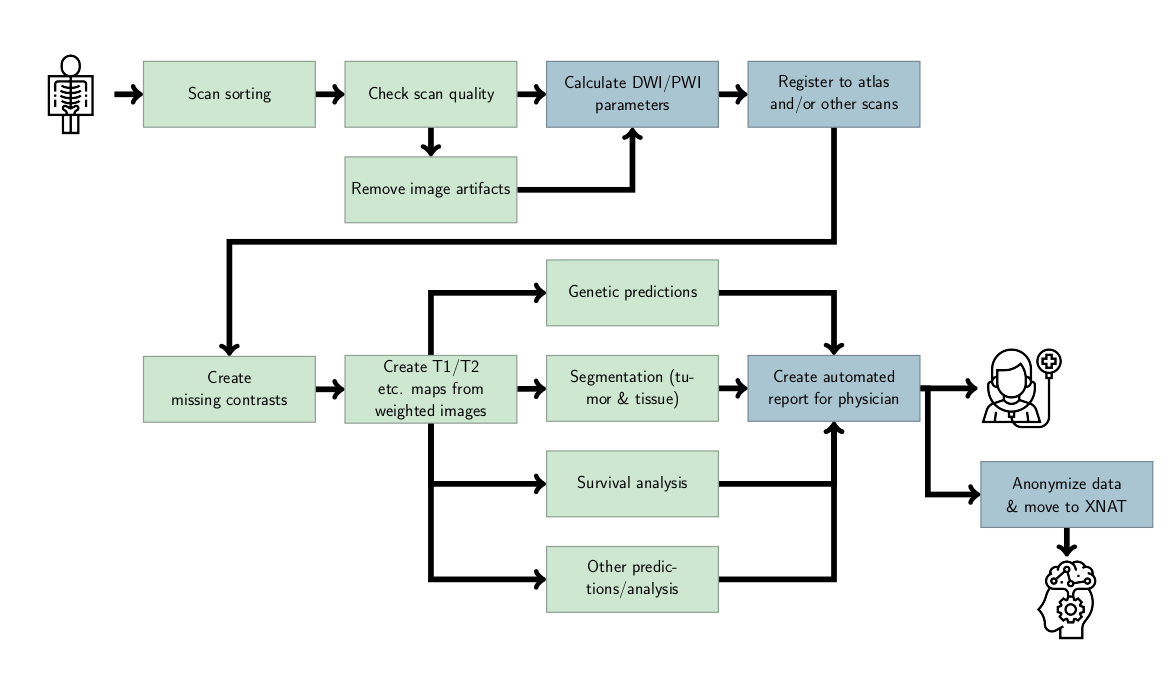
\includegraphics[width=\textwidth]{Figures/Pipeline.png}
\caption{Overview of some steps in which automated or machine learning methods can play a role from the scanner till the scan reaches the clinician}\label{fig:discussion_pipeline_automatic}
\end{figure}

The radiomics predictions might also be reconsidered.
For example, instead of predicting genetics, it might be more interesting to predict which parts of the \gls{tumor} are the most important to remove during the resection.
This is information that is currently not available from a ground truth model, and thus provides truly new information.
In the same way, methods could be developed that can help to determine the best course of treatment for a certain patient.
Although these types of research will be faced with methodological challenges, right now the most important step it to reach a clinical consensus, to ensure that the field of radiomics is pushed in the right direction.

All in all, radiomics and automated image analysis are definitely here to stay.
With the increasing healthcare costs, the increasing amounts of data, and the decreasing amount of time clinical experts can spend on a single patient, automatic methods offer a cheap solution that can easily deal with large amounts of data.
Although several methodological and social barriers still need to be overcome, the ultimate goal of improved patient healthcare should be kept as the focus both from the technological side, and from the clinical side.
Ultimately, we do need to move away from the human eye to more objective analysis methods, while at the same time making sure that these automated methods provide the information clinicians want and that the automated methods and clinical experts can see eye to eye about each other's value.
